\documentclass{standalone}
\usepackage{tikz}
\usetikzlibrary{shapes, arrows.meta}

\begin{document}
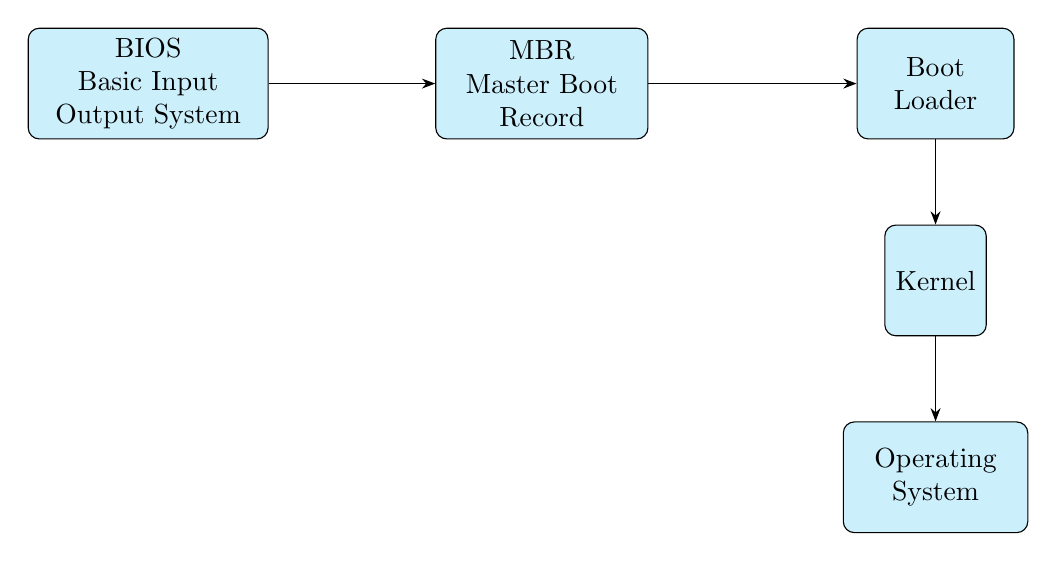
\begin{tikzpicture}[node distance=2.5cm, auto]

    % Styles
    \tikzstyle{block} = [rectangle, draw, fill=cyan!20, 
        text centered, rounded corners, minimum height=4em]
    \tikzstyle{line} = [draw, -{Stealth[scale=1.0]}]

    % Nodes with specified text width
    \node [block, text width=8em] (bios) {BIOS\\Basic Input Output System};
    \node [block, text width=7em, right of=bios, node distance=5cm] (mbr) {MBR\\Master Boot Record};
    \node [block, text width=5em, right of=mbr, node distance=5cm] (bootloader) {Boot Loader};
    \node [block, text width=3em, below of=bootloader] (kernel) {Kernel};
    \node [block, text width=6em, below of=kernel] (os) {Operating System};

    % Paths
    \path [line] (bios) -- (mbr);
    \path [line] (mbr) -- (bootloader);
    \path [line] (bootloader) -- (kernel);
    \path [line] (kernel) -- (os);

\end{tikzpicture}
\end{document}
